\documentclass{article}


\usepackage{graphicx}
\graphicspath{ {"C:/Users/cvg11/Desktop/proj/elec-inspec-protec/report_images"} }



\title{Redistricting Ideology}


\author{
  Drew Keller \\
  Alejandro Navarrete \\
  Victor Perez Martin \\
  Evelyn Siu \\
  Cole von Glahn \\
  The University of Chicago
  Computational Analysis and Public Policy
}

\begin{document}
\maketitle{}


\begin{abstract}
    Political redistricting is a fraught process with high potential for abuse, which is exacerbated by the increasing availability of voter data and computational tools including machine learning. Given this situation, we wanted to explore the potential for machine learning to help shed transparency on the redistricting process. As a first step towards this goal, in this project we used demographic data to train several models to predict the ideological character of precincts in Michigan, as estimated from 2018 election data. We achieved a maximum accuracy of roughly 80 percent using a random forest to predict categorical precinct labels, or R-squared = 0.62 using a Light Gradient Boosting Tree to predict precinct weighted ideology scores.
\end{abstract}


\subsection{Motivation}
  Partisan redrawing of voting maps in the United States is a central strategy for collecting and 
  maintaining political power for one party when it is meant to be about ensuring political representation and participation of the citizenry.
  With every collection of census data per decade, the districts for congressional representation must be revised to accommodate shifts in population proportions while maintaining political competition. 
  Advances in algorithmic tools for this purpose foreshadow a 
  deepening and hardening of ideological bastions and a shift from the purpose of redistricting. 
  Should we prepare a response to this potential future, it would require an understanding of the relationship between voters and their ultimate representative ideology.
  Furthermore, representative ideology would also be a function of the area's vote split between the top candidates for office. 
  To investigate how the shifts in demographics leads to changes in an area's representative ideology and election outcomes, we would need to link precinct demographics to candidate ideologies through vote share. This provides a proxy for the 
  ideological spectrum at the precinct level. Feeding this information through predictive models
  predicated on redrawn voting district maps expresses the expected ideological score of a given
  district, and therefore, the anticipated ideological position of the most appropriate representative.
  Analyzing the difference between these predictions and future outcomes provides the public with a window 
  into the extent to which their beliefs and interests are being accurately represented by their
  Congressperson.
\end{abstract}


\section{Datasets}


Our work leverages data from the following three datasets. 
\begin{itemize}
    \item American Community Survey 5-year estimates, 2018
    \item DIME candidate ideology scores
    \item Precinct-level voter results

\subsection{Candidate Ideology Scoring}


Stanford’s Database on Ideology, Money, and Elections (DIME) includes candidate ideology scores. These scores are assigned based on the ideological positions of the candidate’s donors, as well as those causes/candidates to which the candidate donates. Scores are provided for candidates who reach the general election. We performed fuzzy matching on candidates’ names to combine election results and ideology scores, we decided to keep only the precincts where all the candidates have a minimum matching score of 70 out of 100. We discarded data points where there was only a Republican or Democratic candidate due to the effect of such a situation on the vote share. 

After the cleaning process, we ended up with a sample of 1,042 precincts, out of the 4,765 precincts identified in the Census, with the respective ideology scores of the candidates that ran for Congress in the 2018 election. Ideology scores are centered around zero, a zero score indicates a moderate ideology, a score above 0 a more conservative leaning ideology, and a score below 0 a more liberal. 

We then calculated “weighted” ideology scores as the dot product of [Republican ideology score, Democrat ideology score] and [Republican vote fraction, Democrat vote fraction]. In addition to this continuous measure, we constructed two alternative categorical labels.

First, for the decision tree and random forest models, we prepared classification labels on two dimensions, such that they indicate a winner (Democrat, Republican), and whether the election was close or not (Close, Split). The election was considered close if the percentage of votes each party received was within 50 percent of each other (inside range of 25-75). If the percentage vote breakdown was outside of this range (outside range of 25-75), the election was considered “split”. These two labels tell us who is predicted to win the election, and whether the outcome is likely to be highly partisan (split) or not.

Second, for the logistic regression models, we prepared classification labels as follows:

\begin{itemize}
    \item Very Liberal if s less than -1
    \item Strong Liberal if s between [-1, -0.5)
    \item Lean Liberal if s between [-0.5, 0)
    \item Lean Conservative if s between [0, -0.5)
    \item Strong Conservative if s between [0.5, 1)
    \item Very Conservative if s greater than or equal to 1
\end{itemize}

Table 1: Ideology Score Class Distribution
\begin{table}[h]
    \begin{tabular}{lll}
    \hline
    Category            & Freq. & Percent \\
    \hline
    Strong conservative & 250   & 10.72   \\
    Very Conservative   & 1,031 & 44.21   \\
    Very Liberal        & 1,051 & 45.07   \\
    \hline
    N                   & 2,332 &    
    \end{tabular}
\end{table}



\subsection{Precinct-Level Voting Results}


2018 US House Election Results at the precinct level data come from Redistricting Data Hub. 
For each precinct, we have the names of the candidates that ran in the 2018 election, 
their political party and the total number of votes they received.



\subsection{Demographic Data}


As redistricting is often focused on voters’ demographics - on which high-quality aggregate data is publicly available -  the intersection of demography and ideology is a window to the strategic decisions being made by candidates and party bodies as they construct political geography. Thus, we decided to use demographic features to train our models.

We obtained estimates of several demographic characteristics at the census block group level from the 2018 American Community Survey (5-year). The characteristics comprised 19 features, all continuous:

\begin{itemize}
    \item Total population and population density 
    \item Fraction of population {non-Hispanic white, non-Hispanic Black, Hispanic, American Indian, Asian}
    \item Fraction of households {married family, non-married family, non-family}
    \item Fraction of population with education {less than high school, high school diploma, some college, bachelors degree, higher education}
    \item Fraction of households with median income {less than $30k, $30k-$50k, $50k-$100k, more than $100k}
\end{itemize}
We did not normalize the features, as all were within [0,1] except total population and population density. We carried out areal interpolation of each feature from Michigan’s 8,205 census block groups to 4,805 precincts, based on the assumption of homogenous population characteristics within each census block group. 

In order to merge the election results with the census information and absent a common precinct identifier in both datasets, we combined the county, minor civil division, ward and precinct codes in the election results data to build an id to mimic the precinct id in the Census. 


\section{Model and Experiment Details}


We created three models to try to optimize  accuracy and interpretability. Each model 
predicts precinct ideology classification or score based on demographic features.

\subsection{Trees and Forests}

We chose a decision tree as our baseline model. To improve upon the decision tree, we used the ensemble method random forest. Because the two algorithms are classification methods, we used the  categorical ideology label to classify our dataset. We varied the tree depth between 1 and the entire feature set hyperparameter to optimize our model. We evaluated these models on accuracy, meaning percent correct classification. Below is a list of the accuracy scores for trees from depth 1 to splitting on all available attributes. 

\includegraphics{tree_score}

\includegraphics{rf_scores}

We also varied splitting using entropy v. gini calculations, but did not see a large difference between the two methods. For the random forest, we ran a repeated k-fold cross-validation, using 10 folds and 3 repeats, and a 70/30 train/test split. The mean accuracy was 0.815 with a standard deviation of 0.040.

Decision trees of depth 1 and 2 had the highest accuracy, 77 percent, both (effectively) splitting only on population density. Intuitively, this makes sense, as we know rural areas are more likely to be Republican, and densely populated cities are more likely to be Democratic. Adding in proportion Black did not affect the accuracy score. Naively, Republican, Close makes up 66 percent of the entire sample, so a 77 percent accuracy is a mild improvement. In terms of feature importance for the decision tree (calculated as the decrease in node impurity), the proportion of the population making more than 100,000 dollars had the highest importance at 54.5 percent, followed by the proportion of the population with some college education at 15 percent.

A random forest with a depth of 5 had the highest accuracy score, at 80.8 percent. This was an improvement over the decision tree. For the forest, total population was weighted the highest, at a score of 12.2 percent, followed by proportion of the population that is white, weighted at 0.9 percent.

This was an improvement over the decision tree. For the forest, total pop was 
weighted the highest, at a score of 12.2 percent, followed by prop white, 
weighted at 0.9 percent. 



\subsection{Logistic Regression}

A logistic regression serves well in the case of using compositional data to predict an outcome. It is very much intuitive and interpretable as a model that applies weights to features to generate probabilities.

In our model, we predicted one multi-class dependent variable (the latter ideology classification method mentioned in 1.1) and two binary dependent variables, party of winning candidate and vote split (how the ticket was split between the top two candidates). Using the multi-output classifier wrapper available in scikit-learn, we could run three multiclass predictions at once to predict a vector of the three variables of interest. This design would allow us to experiment with predicting all three outcomes independently and see if those outcomes can thus be predicted on the precinct demographics on their own. 

With this data-set, to avoid multicollinearity in our compositional data, we removed one of the variables from each grouping of proportions. We removed the variables measuring the proportions of white, single, post-secondary graduates with income over 100,000 dollars. These dropped variables would then be the baseline from which to interpret the model. Given that we used a model that does include a bias/intercept, the weights given to all the remaining attributes would show shifts from the baseline. In other words, how much those attributes shift the probabilities of these outcomes away from that expected of a precinct composed only by those characteristics from the omitted group.

Since this classifier is an ensemble of three classifiers, one accuracy metric would be an all or nothing measure. This would see if all values in the predicted outcome vectors match with the true outcome vectors. If not, then that prediction would be marked incorrect. Another metric would be to calculate an average accuracy across all three outcomes.

To investigate the relatively low values of the mean accuracies, 
we experimented with two alternatives. 
First, we manipulated the number of iterations to see if the learning algorithm required more iterations to converge.


Next we used a chaining ensemble method to possibly increase the accuracy where two of the three results may be more probable in conjunction with each other. The first did not improve outcomes. The second reduced mean accuracy and maintained total outcome accuracy.


To conclude, the logistic regression on this dataset was better than random classification for all three values and highly accurate on each independent outcome variable. However, a conjunction of multiple, multiclass classification does not perform as well as the tree-based models.

Table 4: Logistic Regression Training and Testing Accuracies
\begin{table}[h]
\begin{tabular}{l|ll}
\hline 
        & Absolute & Average \\
\hline
Training & 61.86    & 85.36   \\
Testing  & 56.57    & 82.74  
\end{tabular}
\end{table}

\subsection{Light Gradient Boosting Tree}

We employed Light's GBM Regressor model to provide a continuous variable alternative
to the classification methods described above. Ideology as a contiuum 
is essential to our analytic paradigm. While it could be estimated by classification
models, it could not be fully represented. Light GBM also yields high accuracy
on relatively small datasets with many features by downweighting the lowest gradient
and most mutually exclusive attributes.

We used the Light GBM regressor to make predictions on voting outcomes as well as
precinct ideology. For voting, our outcome variable was the percent of votes for the
Democratic candidate. For ideology, our outcome variable was the ideology of all
candidates in the field weighted by their vote share within the given precinct.

Our primary hyperparameter tuning involved the learning rate. We tested learning rates
iteratively on both outcome variables, finding slightly different optimal rates for each.
We measured success of this model through the R-squared value to show the model's
efficacy in explaining variance relative to inputs.

The tables below shows the features sorted by importance as well as the R-squared values
for both model outcomes.

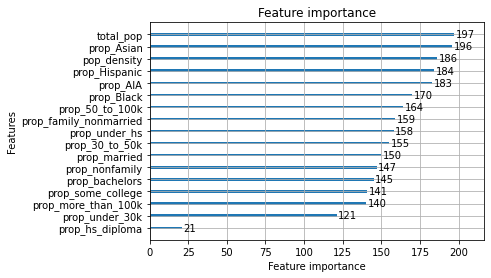
\includegraphics{perc_dem_feat_imp}

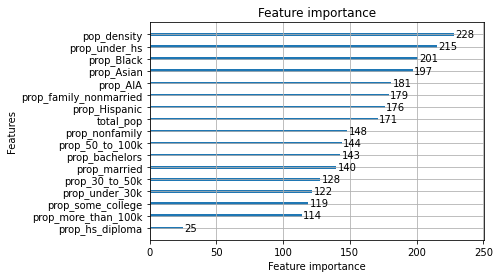
\includegraphics{weight_feat_imp}

In summary, Light GBM effectively explained the variation in both cases. However, it was
stronger with the ideology mapping. Further tuning and larger datasets could improve performance. 
These results are encouraging, as the primary purposeof employing GBM is to best model the
continuous spectrum of voter belief, whereas the classification prediction regarding winner
is better handled by classifiers like trees and logistic regressions. That said, a future
iteration of this project may benefit from employing GBM classifier models as comparison to
the other classifiers.

\section{Limitations}

We expect our analysis to be limited by the following factors:

Small/Limited Dataset
\begin{itemize}
    \item The DIME dataset is missing a small number of candidates. Moreover, we were unable to successfully match candidates to a majority of precincts in Michigan, which limited the size of our dataset and possibly the external validity of our model, depending on what the characteristics were of excluded precincts. The fact that the Census Bureau does not label their geographic units in the same way as our other datasets may have worsened this matching challenge.
\end{itemize}
Ideology Label Issues
\begin{itemize}
    \item The DIME dataset is a rough estimate of ideology, relying on 3rd party contributors as measurement. It has the advantage of representing more candidates who received votes, thereby increasing our ability to understand the granular aspects of precinct voting preferences. However, it may be a less precise metric than scoring systems that narrow their scope to election winners and label politicians based on their voting records.
    \item At a more general level, using candidate ideology as a proxy for population ideology could be problematic; there is some risk of circular reasoning in trying to assess if politicians are “representative” of a district population’s ideology when that ideology is based on the ideologies of the candidates themselves! In particular, we use general election candidate ideologies which may not well represent the actual ideological characteristics of the population prior to candidate selection and party primaries. Furthermore, ideological distributions are not necessarily fixed over time even in the same population.
\end{itemize}
Lack of feature predictive power
\begin{itemize}
    \item In our reading, and as shown in some of our results, aggregate demographics are not a sufficient set of features for predicting ideological distributions (even an optimal classifier would likely have significant error using demographic information). This is especially true at the regional/state level where the number of observations is limited. Finally, it’s important to note that sampling and nonsampling error and lag in the collection of Census demographic data could impact our analysis.
\end{itemize}


\section{Negative Societal Impacts}

There is the potential that this work is used by political operatives to
further understand and abuse differences in ideology and demography. Rather
than a tool for changing candidate behavior and encouraging a closer match of
representative to represented, it may be leveraged to instead alter the playing
field in favor of particular candidates and their ideological beliefs.


\section{Conclusion}

While the baseline categorizations of the decision tree and logistic regression produce moderately accurate estimates of district ideology, the random forest and gradient boosted decision tree models provide more effective means of determining both the voting outcomes and ideological makeups for precinct specific voter behaviors. These measures give policymakers the opportunity to assess the impact of redistricting on representation accuracy. If a district’s aggregated ideological outcomes differ greatly  from voting outcomes, it could be a sign that the particular needs of that community are not accurately represented at the legislative level. That knowledge can reveal roadmaps for improving the health of representative democracy. More importantly it can provide communities with an understanding of how likely their needs are to be met, and the extent to which their beliefs are fought for on the national stage.



\section{Asset Attribution}

\begin{itemize}

\item Bonica, Adam. 2019. Database on Ideology, Money in Politics, and Elections: Public version
3.0 [Computer file]. Stanford, CA: Stanford University Libraries. <http://data.stanford.edu/
dime>.

\item Bonica, Adam. 2018. “Inferring Roll-Call Scores from Campaign Contributions Using Super-
vised Machine Learning” American Journal of Political Science, 62, (4): 830-848. (onlinelibrary.wiley.com/doi/full/10.1111/ajps.12376).

\item U.S. Census Bureau. (2012). 2020 American Community Survey.  
Retrieved from https://www.census.gov/data/datasets.html.

\item Voting and Election Science Team, 2019, "2018 Precinct-Level Election Results", 
https://doi.org/10.7910/DVN/UBKYRU, Harvard Dataverse, V59.

\end{itemize}

\end{document}